\section{Related Work}
\label{sec-related}

We organize the related work surrounding efficient, low-cost memory protection
techniques in two separate sections : \textbf{memory encryption} and
\textbf{memory integrity verification}.

\subsection{Memory Encryption}
The goal of memory encryption is to protect the confidentiality of
sensitive information from unauthorized subjects. Sensitive information
includes but is not limited to: secret keys, secret code (e.g. proprietary boot
code) and private data. The \TT{National Institute of Standards and Technology}
(NIST) actively regulates the encryption standards. Recently, two symmetric key
cryptographic algorithms are being increasingly used in trusted hardware
computing : Triple Data Encryption Standard (3DES) and Advanced Encryption
Standard/Rjindael (AES). As AES provides systems with a higher minimum security
strength, it is more widely used in recent hardware accelerated trusted
computing studies as compared to 3DES. For instance, Intel has developed
extensions to it's instruction set architecture (ISA) to enable fast encryption
and decryption using AES. The studies in this survey mainly focus on using AES
to develop efficient, low-cost encryption and decryption modules.

%%%%%%%%%%%%%%%%%%%%%%%%%%%%%%%%%%%%%%%%%%%
\subsubsection{AES Counter Mode Encryption}
%%%%%%%%%%%%%%%%%%%%%%%%%%%%%%%%%%%%%%%%%%%
AES supports three general modes of operation: Electronic Codebook (ECB),
Cipher Block Chaining (CBC) and Counter (CTR). Since the AES-ECB mode preserves
patterns from the plaintext to the ciphertext, it does not provide adequate
confidentiality protection. Both AES-CBC and AES-CTR eliminate this information
leak by chaining the encryption between individual AES encryption blocks
(16-bits). This however precludes users from encrypting and decrypting blocks
in parallel (as supported by AES-ECB). As discussed in \cite{suh-memIntEnc},
decrypting the ciphertext stored in memory can drastically increase the load
use delay latency of processing systems. The added latency is a result of the
serial memory fetch then decrypt memory block operation. To hide this latency
Suh et. al. use a \TT{one-time pad} (OTP) based encryption / decryption
technique. The OTP is generated by encrypting the plaintext under a a secret
key using AES-CTR with the following equation:

$$\TT{plaintext} = {\TT{FV} || \TT{Addr} || \TT{TS} || \TT{i}}$$

In the equation above, \TT{FV} is a fixed vector, \TT{Addr} is the memory
address being accessed, \TT{TS} is a timestamp stored along with the encrypted
data and \TT{i} is the block number.  The use of a monotonically incrementing
counter, \TT{TS}, ensures the uniqueness of the \TT{OTP} - proven to be
cryptographically secure. Generating the \TT{OTP} using this method enables the
system to overlap the AES-CTR decryption latency with the memory fetch /
accessing latency \cite{suh-memIntEnc}. To mitigate the fetch latency, Suh et.
al. also mentions the \TT{TS} values can be cached latency to better hide the
AES-CTR decryption latency. This method reduces the load-use-delay latency to
the latency of performing an $\oplus$ between the generated \TT{OTP} and
encrypted data.

%%%%%%%%%%%%%%%%%%%%%%%%%%%%%%%%%%%%%%%%%%%
\subsubsection{AEGIS}
%%%%%%%%%%%%%%%%%%%%%%%%%%%%%%%%%%%%%%%%%%%
Furthering the AES-CTR based decryption \cite{suh-memIntEnc}, AEGIS
\cite{aegis} adds low-level OS-kernel support to provide additional
confidentiality features. That is, AEGIS is a single-chip secure processor that
leverages OS-kernel modes to provide additional encryption (ME mode) and
integrity-verification (IV mode) features. The OS also manages four distinct
protected regions in virtual memory:

\begin{enumerate}[noitemsep, topsep=0pt]
    \item Read-only (static) verified memory
    \item Read-write (static) verified memory
    \item Read-only (dynamic) private memory
    \item Read-write (dynamic) private memory
\end{enumerate}

These modes help isolate the virtual memory space of each process to ensure
that secret keys are kept confidential across multiple users and between users
and the supervisor. AEGIS also employs physically random functions (also known
as physically unclonable functions) to generate secret keys as they are less
prone to physical hardware attacks than the alternatives such as using
non-volatile memory (e.g. EEPROM) and fuses.

%%%%%%%%%%%%%%%%%%%%%%%%%%%%%%%%%%%%%%%%%%%
\subsubsection{Improving Encrypted Memory Performance}
%%%%%%%%%%%%%%%%%%%%%%%%%%%%%%%%%%%%%%%%%%%
The previous two studies \cite{suh-memIntEnc} \cite{aegis} illustrate the
fundamental AES-CTR generated \TT{OTP} encryption scheme and OS kernel based
memory isolation schemes. Though these studies provide the basic building
blocks for memory encryption, they do not address the challenge of minimizing
power, performance and durability overhead when writing encrypted segments to
memory. Traditionally, plaintext \TT{writes} to memory only change 12 \% of
destination block's  bits \cite{duece}. According to the \TT{Avalance Effect}
\cite{avalance} changing a single plaintext bit causes 50 \% of the
ciphertext's bits to change. For instance, changing the most significant bit in
the plaintext should cascade the change to every encryption block in the
AES-CTR chain. This is a desired property when using cryptographic encryption
algorithms; changing a single plaintext bit should cause the ciphertext to
appear completely ``random''. In comparison to writing plaintext data,
encrypted data causes 4x as many bits to flip in memory.

Many modern memory systems use more efficient write schemes such as \TT{Data
Comparison Write} (DCR) \cite{dcr} and \TT{Flip-n-write} \cite{fnw} (FNW) to
take advantage of the fewer overridden plaintext bits. Techniques such as DCR
and FNW however, only work when writing plaintext data to memory. For instance,
FNW bounds the number of bit flips to a maximum of half the number of bits per
line. Such optimizations limit the number of modified bits to only 10 \% to 15
\% on average. This greatly improves write performance and durability of
limited-endurance memory such as non-volatile memory (e.g. PCM). Unfortunately,
these optimizations are not amenable to encrypted data when 50 \% of the bits
change on average - increasing power, reducing durability and reducing write
bandwidth. Dual Counter Encryption (DUECE) \cite{duece} is one solution to
write-efficient encryption.

DUECE makes the observation that only a few words are changed during each write
operation so only the changed words need to be re-encrypted. DUECE maintains a
leading (LCTR) and trailing (TCTR) counter for each cache line as well as an
encryption time slot : \TT{Epoch}. An \TT{Epoch} is defined as four writes to
the cache. Within the \TT{Epoch} interval, modified words are encrypted using
the LCTR. At the \TT{Epoch} boundary, the entire line is re-encrypted under a
new counter, \TT{LCTR = TCTR}. In order to reduce the storage space requried by
LCTR and TCTR, the TCTR is computed by masking a pre-determined number of
least-significant bits of the LCTR. The pre-determined number of bits make up a
\TT{wordsize}. The \TT{Epoch} and \TT{wordsize} must be carefully chosen to
optimize the bit flips, full encryption overhead, storage overhead and fineness
of tracking modified words in cachelines. DUECE performs well when programs
write to cachelines in sparse and regular patterns. DUECE reduces the number of
bit flips for encrypted memory writes by a factor of 2 (from 50 \%
to 24 \% bit flips) \cite{duece}.

DUECE also has the option of enabling a DynDUECE operating mode.  DynDUECE
allows the write scheme to dynamically switch from DUECE to FNW if the program
modifies all the words in a specific cache line. In the case of denser memory
writes, FNW is able to reduce bit flips of encrypted memory by 14 \%
\cite{duece}. The dynamic switching between DUECE and FNW also only incur a 1
bit overhead per cacheline.

Finally, DUECE employs a novel \TT{Horizontal Wear Leveling} technique to
evenly distribute the writes across words in a cacheline. In programs with
regular memory access patterns, it is often the case that some words in a cache
line are accessed more frequently than others. This causes differential
hardware wear leveling on the memory units - which is more pronounced in
non-volatile memory architectures such as PCM. To mitigate wear leveling DUECE
employs an efficient horizontal wear leveling technique that uses algebraic
functions to calculate rotation levels. Overall, DUECE is able to drastically
improve write throughput as well as overall system performance while reducing
the energy delay product (EDP).

%%%%%%%%%%%%%%%%%%%%%%%%%%%%%%%%%%%%%%%%%%%
\subsubsection{Galois Counter Mode Based Encryption}
%%%%%%%%%%%%%%%%%%%%%%%%%%%%%%%%%%%%%%%%%%%
In addition to using AES-CTR mode encryption, some studies have investigated
the use of Galois/Counter Mode (GCM) encryption: a highly parallel and
efficient block cipher mode that supports authenticated encryption
\cite{nistGCM}. GCM is similar to AES-CTR mode in that it can be used to
generate \TT{OTP}s. Yan et.  al developed a GCM based encryption method that
uses a split counter comprising of a major and minor counter \cite{gcmMem}. The
major counter is common over an encryption page and a minor counter is
maintained for each block. The minor counter requires an additional 8 bits for
each 64 bits. This study will be discussed more in the following section.

%%%%%%%%%%%%%%%%%%%%%%%%%%%%%%%%%%%%%%%%%%%%%%%%%%%%%%%%%%%%%%%%%%%%%%%%%%%%%%%
\subsection{Integrity Verification}
%%%%%%%%%%%%%%%%%%%%%%%%%%%%%%%%%%%%%%%%%%%%%%%%%%%%%%%%%%%%%%%%%%%%%%%%%%%%%%%
The goal of memory integrity verification is to protect the integrity of
memory and detect corrupted memory. Generally, the protection mechanism must be
able to detect when memory is maliciously changed. That is, when a processor
reads from memory it should get the last version of the data that was written.
Over the years a few main cryptographic integrity verification
algorithms have been developed including : Hashes and Message Authentication
Code (MAC). The first strategy in providing integrity verification involves
storing either a hash or MAC generated tag with each memory block of the
off-chip memory.  The hash or MAC is computed and stored during write
operations and verified during read operations. The hash (128 bit) based
approach incurs a 25 \% memory overhead and the MAC (64 bit nonce) incurs a
12.5 \% memory overhead for standard 512-bit cache line off-chip memory
authentication \cite{surveyInt}.  The previously discussed authentication
techniques provide memory authentication mechanisms at a high cost in terms of
off-chip memory overhead.  The following sections focus on discussing
\TT{Integrity Trees} which aim to reduce the memory overhead required to
provide integrity verification for off-chip memories.

\subsubsection{Integrity Trees}

The first approach to using integrity trees for off-chip memory authentication
is Merkle trees \cite{merkle}. A Merkle tree is a tree of hashes as shown in
Figure \ref{fig:intTree}a.

\begin{figure}[!htb]
  \centering
  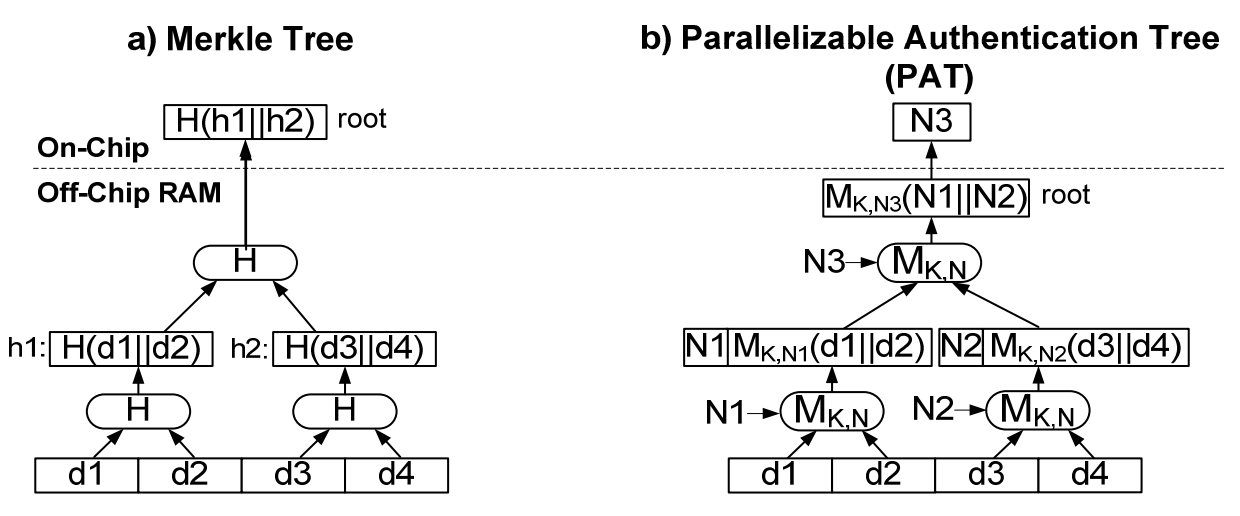
\includegraphics[width=0.5\textwidth]{figs/integrityTrees.PNG}
  \caption{H: Hash Tree. M: MAC function. $d_y$ : data block y. $N_z$: Nonce z.
  K : Secret Key.\cite{surveyInt}}
  \label{fig:intTree}
\end{figure}

The \TT{integrity check} or \TT{verification} operation performed during a
memory read operation can be parallelized for a Merkle Tree however, updating
the tree is a sequential process that must be performed from the leaves up to
the root. Qualitatively, the Merkle tree reduces the \TT{integrity check} from
a growing linearly with respect to the number of memory blocks to growing
logarithmically. There has been work in reducing the architectural overhead of
\TT{integrity check} operations including optimizing the arity of the hash
tree, the granularity of the authentication check blocks and maintaining a
cache for the hash tree to improve the ``hash fetch'' rate. In general these
techniques tend to be complicated and require significant hardware
enhancements. For instance, aggregating the hash and data caches into a single
monolithic cache can increase miss rates and cache pollution - degrading the
overall system performance.

As seen in Figure \ref{fig:intTree}b, the Parallelizable Authentication Tree
(PAT) \cite{patTree} is an alternative to Merkle trees. Unlike Merkle trees,
PATs overcomes the issue of non-parallelizable integrity tree update operation
during memory write operations by using MACs for providing authentication
instead of hash functions \cite{surveyInt}. The parallelizability of the
integrity tree update does come at a memory storage cost - PAT tree generally
requires $\frac{3}{2}$ the amount of memory that Merkle trees require.

\subsubsection{Log Hash Tables}
As discussed earlier, Merkle trees and PATs maintain hashes or MAC tags for
authenticated memory blocks. Suh et. al. adopt an alternative approach using a
log based hash table to provide memory integrity. In stead of maintaining a
hash for each memory block, a log of memory operations is generated to maintain
a snapshot of the system \cite{suh-memIntEnc}. A separate read and write log is
maintained with minimal runtime overhead so the processor can verify the
integrity of \textit{sequence} of operations later in time
\cite{suh-memIntEnc}. This is considered \TT{lazy} memory integrity management
as the \TT{integrity check} is not performed for every read operation but
rather less frequently - the intervals of performing \TT{integrity check}
operations is much longer. That is, the system would detect a
corrupted memory much after the physically attack took place and maliciously
tampered with the memory. The hash log is shown to be more performance
efficient while incurring a lower memory space overhead than the cached hash
tree approach discussed earlier.

\subsubsection{AEGIS}
As discussed in the memory encryption section, AEGIS is a single-chip secure
processor that provides both memory encryption and integrity verification
mechanisms. AEGIS leverages Physically Random Functions (PRF), sometimes called
Physically Unclonable Functions (PUFs), to provide off-chip memory protection.
AEGIS also uses the OS-kernel modes to provide additional integrity
verification (IV) features. AEGIS allows programs to overlap memory encryption
(ME) and IV stages together, or keep them separate, in order to maximize
flexibility and provide tamper-resistant off-chip memory protection
\cite{suh-memIntEnc}.

\subsubsection{Galois/Counter Mode Integrity Verification}
In addition to using hash and MAC based authentication schemes, some studies
investigate the use cryptographic authenticated encryption algorithm such as
GCM to provide memory integrity verification \cite{gcmMem}. GCM relies on GMAC
/ GHASH function to provide authentication capabilities. GMAC / GHASH functions
are less computationally intensive and incur lower latency overheads compared
to hash algorithms such as MD-5, SHA-1 and SHA-2. Like the AES-CTR mode and GCM
based encryption mechanisms, the memory fetch latency can be used to hide the
GMAC / GHASH functions. The GMAC / GHASH functions generate \TT{OTP}s that are
$\oplus$'ed with the plaintext data to make the tags that will be checked on
memory read operations. By hiding the \TT{OTP} generation latency with memory
fetching, the GMAC / GHASH functions incur very little latency overhead to the
overall system. In order to further improve performance, Yan et. al. also
parallelized the Merkle tree \TT{integrity check} operation \cite{gcmMem}.

\subsubsection{Multi-Core Integrity Verification}
Where the previous studies and techniques focused on single-core
tamper-resistant memory protection, Shi et. al. investigate memory encryption
and integrity verification techniques for multi-core systems
\cite{multicoreEnc}. Shi et. al discuss how Merkle tree (and similarly PATs and
log hash tree) approaches alone do not work for multiprocessor systems.
Additional hardware or software support must be provided to correctly implement
memory encryption and integrity verification. For instance, processes running
on separate cores must not be allowed to access and modify the same memory
integrity trees otherwise the false appearance of malicious memory corruption
could be detected by the \TT{integrity check} operations. Shi et. al. instead
use a single global MAC tree managed by the memory controller and rely on a
secure OS kernel to manage private session keys across cores for specific
user and supervisor processes. The session keys are used to generate unique
secret keys used in the MAC based memory integrity verification.
